\documentclass[12pt,oneside,ams,a4paper]{hepthesis}
\usepackage{polyglossia}
\setmainlanguage[babelshorthands=true]{german}
\setotherlanguage[variant=british]{english}
\usepackage{hfoldsty}
\usepackage{amssymb}
\usepackage[numbers]{natbib}
\setcitestyle{square}
\usepackage{pdfpages}
\usepackage{url}
\usepackage{ulem}
\usepackage{color}
\usepackage[squaren]{SIunits}
\usepackage{upgreek}
\usepackage{hyperref}
\usepackage{braket}
\usepackage{nameref}
\usepackage[section]{placeins}
\KOMAoption{numbers}{noenddot}
\usepackage{booktabs}
\usepackage{datetime}
\usepackage{fontspec}
\usepackage{titling}
\usepackage{glossaries}
\usepackage{fixltx2e}
\usepackage{blindtext}
\usepackage{geometry}
\usepackage{setspace}
\setstretch{1.241}
%\doublespacing{}
\geometry{a4paper,left=20mm,right=20mm}
\author{Malte Zietlow}
\title{Analyse von OAuth 2.0 und OpenID Connect zur Weiterreichung der
\mbox{zwei-Faktor Authentifizierung} aus der TK-App an Meine~TK.}
\date{\today}
\hypersetup{
 pdfauthor = {\theauthor},
 pdftitle = {\thetitle},
 pdfsubject = {Transferleistung, Techniker Krankenkasse/Nordakademie, 2018},
 bookmarksopen=true
}
\raggedbottom{}
\setmainfont[Path=C:/Windows/Fonts/]{times.ttf}
\begin{document}
\newcommand{\theLocationAndDate}{Hamburg, den \thedate}
\renewcommand*\chapterheadstartvskip{\vspace*{-2cm}}
\renewcommand*{\figurename}{Abb.}
\renewcommand*{\figureautorefname}{Abb.}
\renewcommand*{\tablename}{Tab.}
\renewcommand*{\tableautorefname}{Tab.}
\renewcommand*{\chapterautorefname}{Kapitel}
\renewcommand*{\sectionautorefname}{Kapitel}
\renewcommand*{\subsectionautorefname}{Kapitel}
\renewcommand*{\equationautorefname}{Gl.}
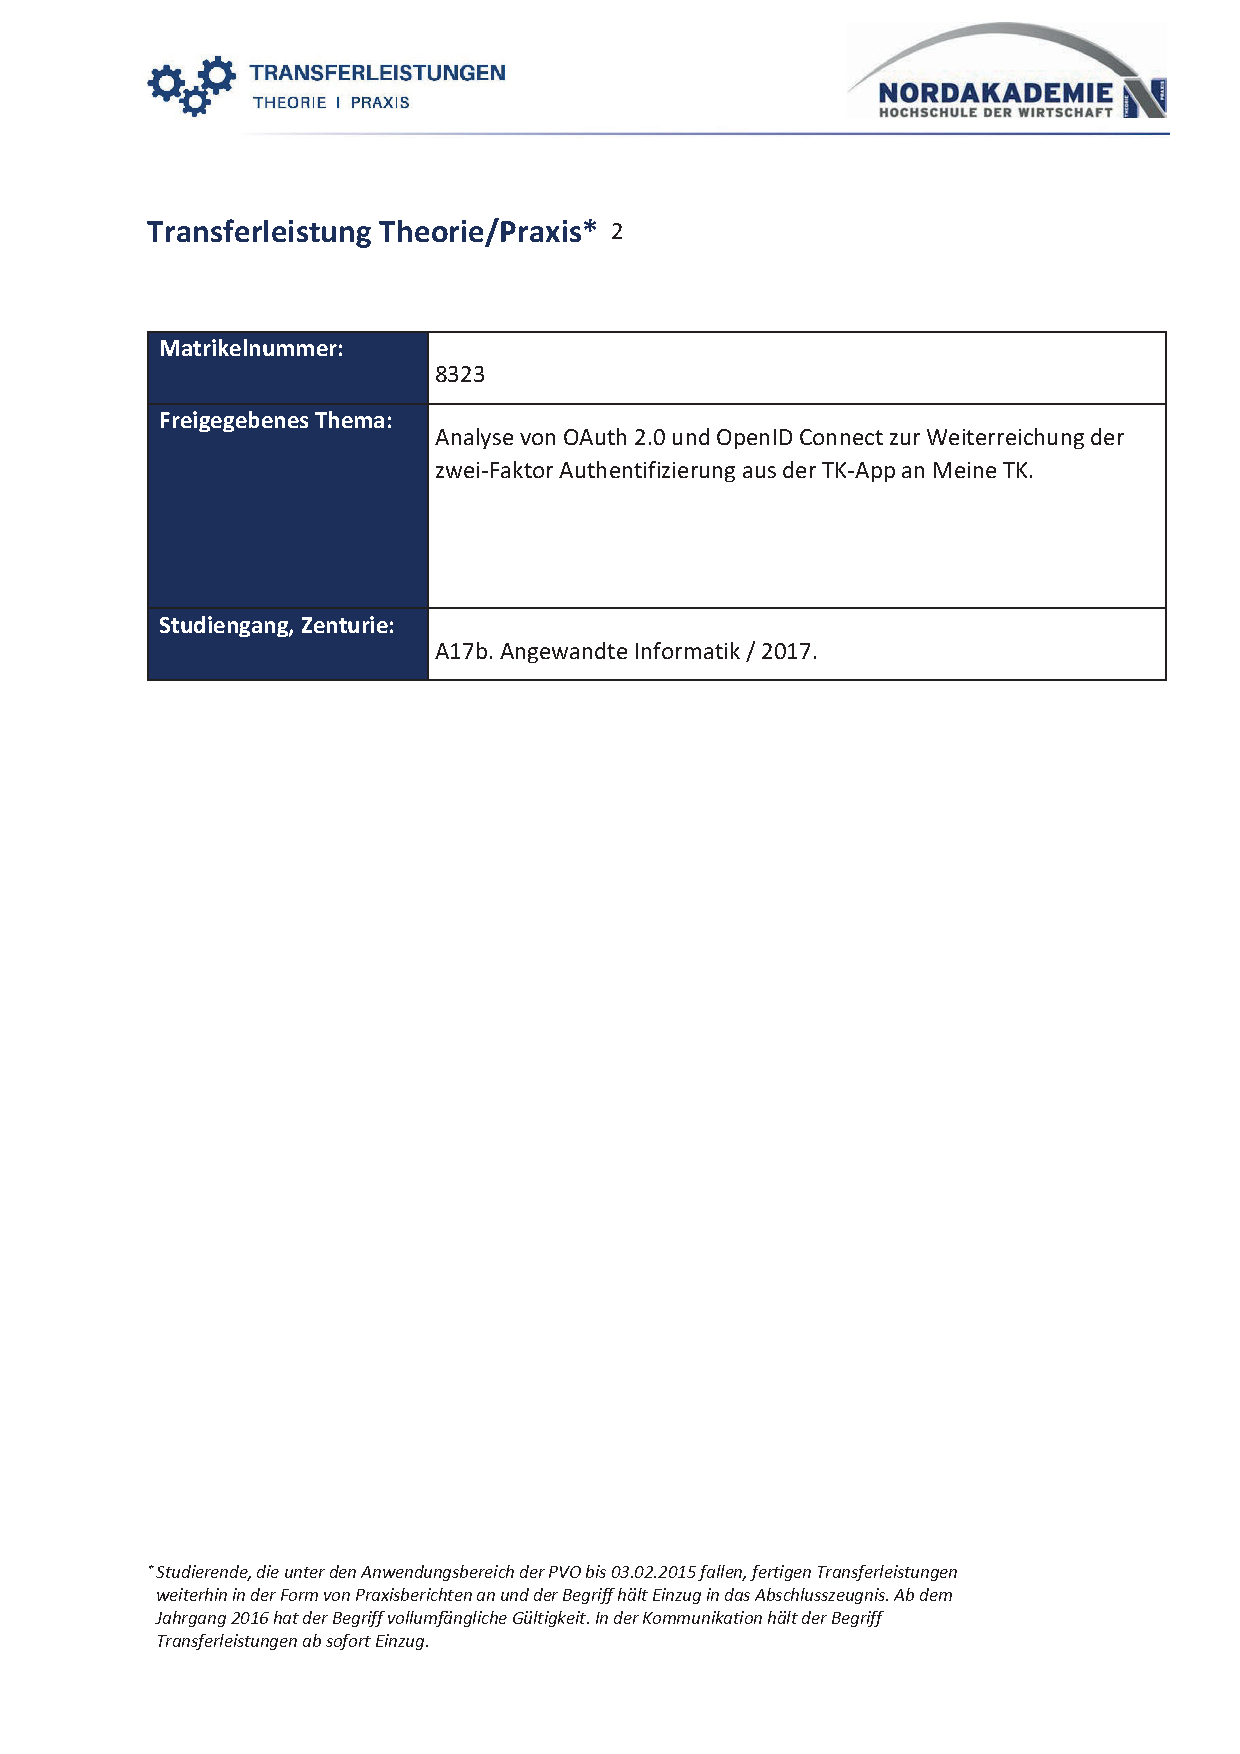
\includepdf[pages=1]{misc/deckblattTerminiert.pdf}
\newpage
\begin{frontmatter}
    \begin{tikzpicture}[remember picture,overlay] \thispagestyle{empty} \node at
(current page.center) {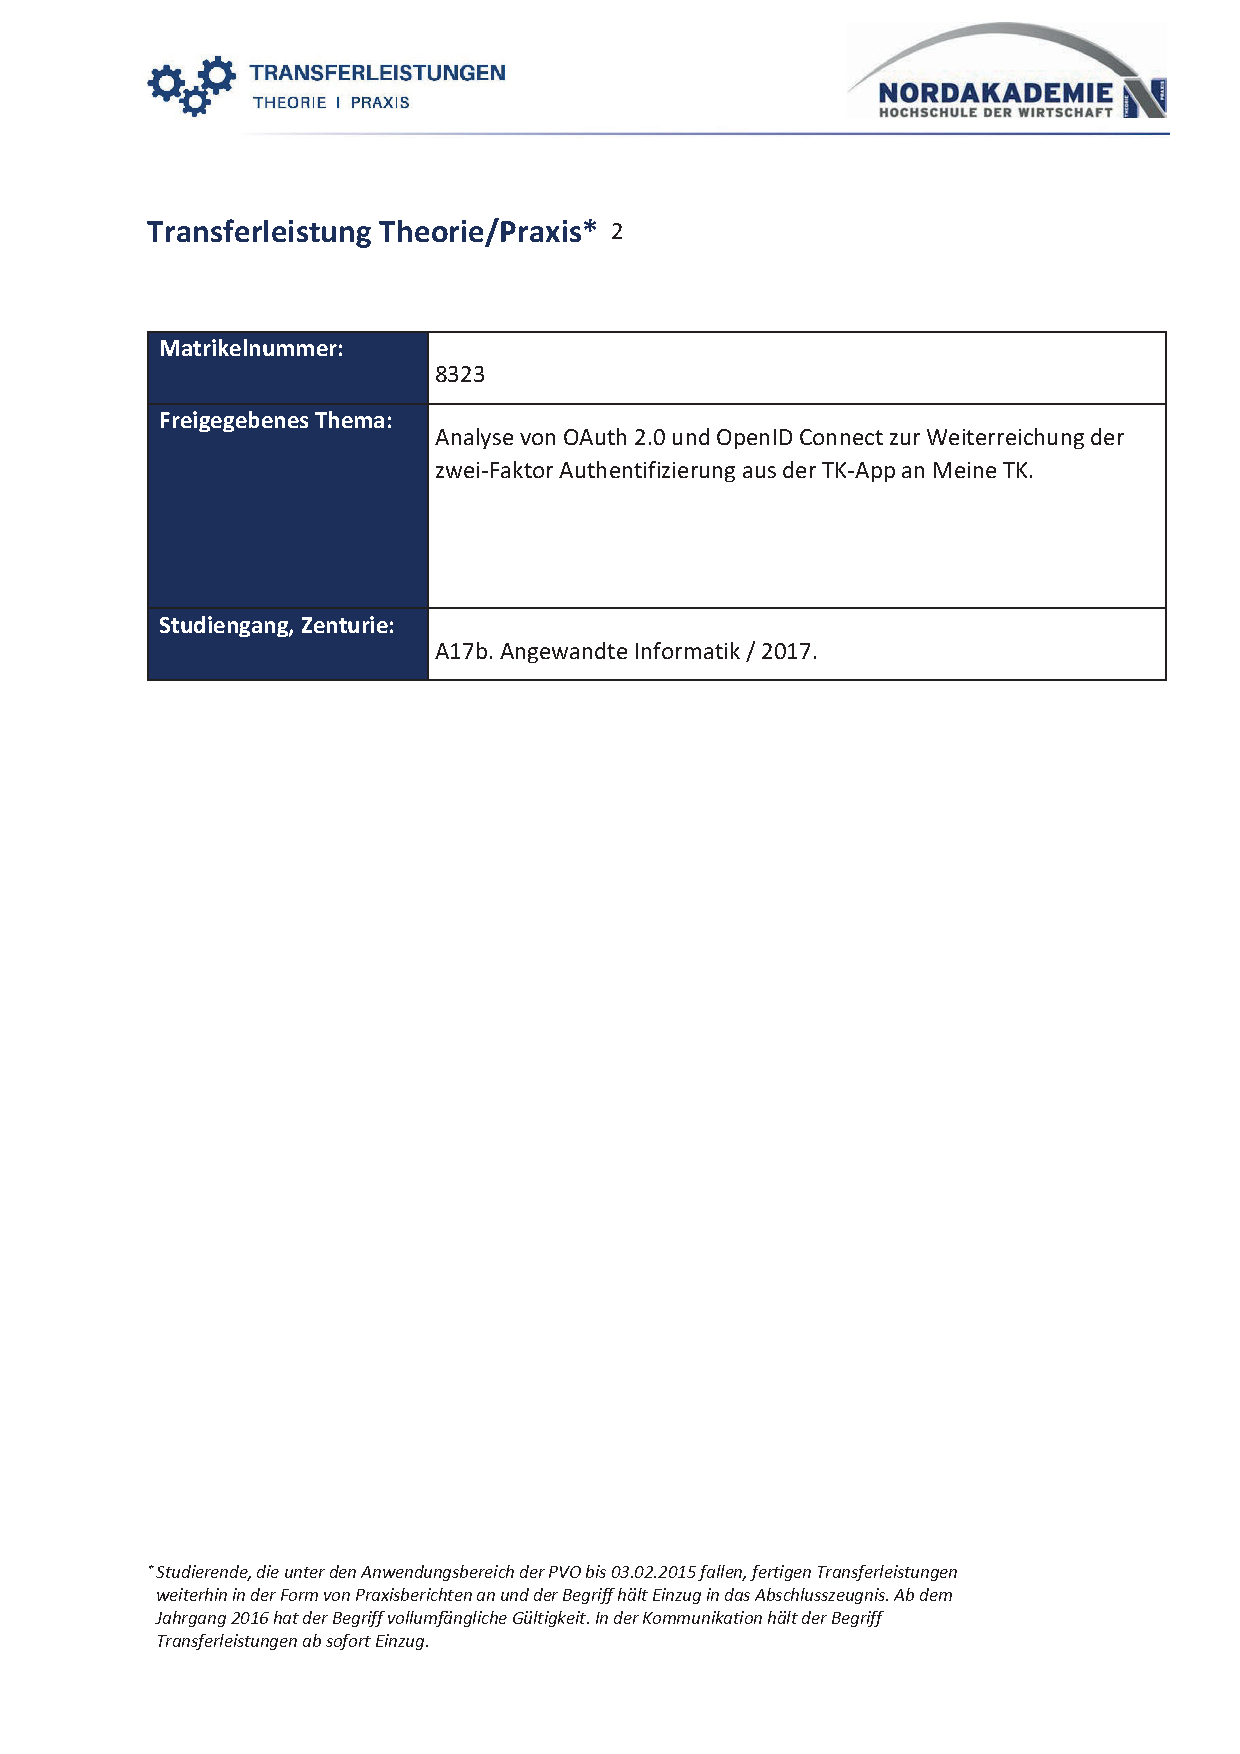
\includegraphics[page=1]{misc/deckblattTerminiert.pdf}};
\end{tikzpicture}
\newpage
% Klassische Titelseite

\thispagestyle{empty}
\begin{center}
\vspace*{-2cm}

\includegraphics[width=0.85\textwidth]{Bilder/Logo_NAK}\\
\vspace*{1.5cm}
    {\titlefont\huge\onehalfspacing{}
	\thetitle{}
    \par}%
\vfill
{
    \normalfont\normalcolor\bfseries\large
    Transferleistung \\
    \large
    im Studiengang Angewandte Informatik\\
    angefertigt im Projekt-Team Innovations.OMP\\
    der Techniker Krankenkasse\\
    \par
}
\end{center}\par
%\vfill
\vspace*{2.5cm}
\noindent\begin{minipage}[b]{\textwidth}
{
  \noindent \textbf{von \theauthor, geb.~am 01.~März 1998 in Bad Oldesloe}\\

  \begin{tabbing}
  \textbf{Betreuer und Prüfer:}  \= \textbf{Jan Koops, Tech-Lead TK-App}
  \\
  \\
  \\
  %\textbf{2. Betreuer und Pr\"ufer:}  \= \textbf{Philip MacDonald, Full-Stack/IOS}\\
  %\textbf{3. Betreuer und Pr\"ufer:}  \= \textbf{Jan Ove Weichel, Android}\\
  \end{tabbing}

  \noindent\textbf{\theLocationAndDate}
}
\end{minipage}

\newpage
\thispagestyle{empty}
\addtocounter{page}{-3}
\setlength{\evensidemargin}{0.6cm} %Zum Drucken -0.6cm Rand einstellen!
\setlength{\oddsidemargin}{0.6cm} %Zum Drucken 0.6cm Rand einstellen!

\begin{abstract}[Kurzzusammenfassung]
\thispagestyle{plain}
\addtocounter{page}{-1}
\fussy
Lorem ipsum dolor sit amet,
consetetur sadipscing elitr, sed diam nonumy eirmod tempor invidunt ut labore et
dolore magna aliquyam erat, sed diam voluptua. At vero eos et accusam et justo
duo dolores et ea rebum. Stet clita kasd gubergren, no sea takimata sanctus est
Lorem ipsum dolor sit amet. Lorem ipsum dolor sit amet, consetetur sadipscing
elitr, sed diam nonumy eirmod tempor invidunt ut labore et dolore magna aliquyam
erat, sed diam voluptua. At vero eos et accusam et justo duo dolores et ea
rebum. Stet clita kasd gubergren, no sea takimata sanctus est Lorem ipsum dolor
sit amet. Lorem ipsum dolor sit amet, consetetur sadipscing elitr, sed diam
nonumy eirmod tempor invidunt ut labore et dolore magna aliquyam erat, sed diam
voluptua. At vero eos et accusam et justo duo dolores et ea rebum. Stet clita
kasd gubergren, no sea takimata sanctus est Lorem ipsum dolor sit amet.

Duis autem vel eum iriure dolor in hendrerit in vulputate velit esse molestie
consequat, vel illum dolore eu feugiat nulla facilisis at vero eros et accumsan
et iusto odio dignissim qui blandit praesent luptatum zzril delenit augue duis
dolore te feugait nulla facilisi. Lorem ipsum dolor sit amet, consectetuer
adipiscing elit, sed diam nonummy nibh euismod tincidunt ut laoreet dolore magna
aliquam erat volutpat.

Ut wisi enim ad minim veniam, quis nostrud exerci tation ullamcorper suscipit
lobortis nisl  \end{abstract}
\setlength{\evensidemargin}{0cm} %Zum Drucken -0.6cm Rand einstellen!
\setlength{\oddsidemargin}{0cm}	 %Zum Drucken 0.6cm Rand einstellen!
\tableofcontents \newpage \thispagestyle{empty}
%\listoffigures
%\listoftables

\end{frontmatter}

\begin{mainmatter}
    \chapter{Einleitung} Seit ungefähr 2016 erprobt die TK Softwareentwicklung in
agilen Teams. Das Team Online and Mobile Projects, in dem diese Arbeit entstand,
ist eines der Pilotprojekte dieses Vorstoßes. Das Team ist unter anderem mit der
Betreuung und Weiterentwicklung der TK-App betraut. Die TK-App versucht,
Verwaltungsprozesse, Kundeninteraktion im Allgemeinen, nutzerfreundlich
umzusetzen.\\ In Meine TK, der Web-Plattform für Versicherte der TK, sind einige
der von uns für die App geplanten Prozesse bereits vorhanden. Teil der agilen
Planung ist das \gls{mvp}. \glspl{mvp} sind minimal nutzbare Produkte. Im Rahmen
eines  \gls{mvp}s ist es denkbar, einen Prozess im ersten Schritt nur teilweise
in der App zu verwirklichen, den Nutzer ab einem bestimmten Punkt an Meine TK
weiterzuleiten und den Prozess dort fortzusetzen. Hierzu müssen Nutzer sich
derzeit stets erneut einloggen. Ziel dieser Arbeit ist, den Prozess der
Weiterleitung für Nutzer angenehmer zu gestalten, indem die erneute Eingabe
seiner Daten für ihn entfällt.\\ Die Weiterleitung von Zugriffsrechten ist seit
2012 mit der Veröffentlichung von \gls{OAuth}
\textit{grundsätzlich} keine schwere Aufgabe mehr. Da die TK jedoch hohe
Ansprüche an ihrer Sicherheitsstandards stellt und die Sicherheit der
Implementierung eines Protokolls nicht durch die Sicherheit des Protokolls
sichergestellt ist, wie~\cite{Sun.2012,Hu.2014,Yang.2016} zeigten, ist diese
Arbeit entstanden.\\ Die Frage, ob sich OAuth, das als Autorisierungsverfahren
gedacht ist, für die Authentifizierung eines Nutzers eignet, wird in dieser
Arbeit elegant umschifft.

\input{Dokument/OAuth/OAuth.tex}
\chapter{OpenID Connect}
\section{Grundlagen}

\section{Flows}

\section{Sicherheitsanalyse}

\section{Fazit}


\input{Dokument/Verdict.tex}
\chapter{Implementation}


\end{mainmatter}

\begin{appendices}
    \chapter{Anhang}

\end{appendices}

\begin{backmatter}
    \addtocontents{toc}{\vspace*{1em}}
% Literaturliste aus Literaturdatenbank (Bibtex-Datei) bauen. Nur tatsaechlich
% zitierte Literatur wird in Liste aufgenommen.

% Regelmaessigen Aufruf von ``bibtex abschlussarbeit'' nicht vergessen, falls
% das der Latex-Editor nicht erledigt.

% Zur Bearbeitung der Literaturdatenbank kann das Programm JabRef
%(http://jabref.sf.net) empfohlen werden. (Java-Programm, laeuft unter Windows,
% Linux, Mac, \ldots)

\bibliography{Literatur/bibtex/Literatur}
% Stil fuer Literaturliste festlegen
% Variante A: DIN, Eintraege erhalten Kuerzel aus Autoren-Initialien und Jahr,
% alphabetisch geordnet

            %\bibliographystyle{alphadin}

% Variante B: DIN, Eintraege werden durchnummeriert, alphabetisch geordnet

            %\bibliographystyle{unsrt}

% Variante C: Harvard.
             \bibliographystyle{agsm}

\newpage
\thispagestyle{empty}
\section*{Selbständigkeitserklärung}
Ich versichere hiermit an Eides statt, dass ich die vorliegende Arbeit
selbstständig angefertigt und ohne fremde Hilfe verfasst habe, keine außer den
von mir angegebenen Hilfsmitteln und Quellen dazu verwendet habe und die den
benutzten Werken inhaltlich und wörtlich entnommenen Stellen als solche
kenntlich gemacht habe. \vspace*{2cm}

\begin{flushright} \theLocationAndDate{} \end{flushright}

\end{backmatter}

\end{document}
